\documentclass[conference]{IEEEtran}
\usepackage{balance}
\usepackage{moreverb}
\usepackage{amsmath}
\usepackage[utf8]{inputenc}
\usepackage{pifont}
\usepackage{listings}  
\usepackage{color}  
\usepackage{textcomp}  
\usepackage{url}  
\usepackage{array}
\usepackage{booktabs}
\setlength{\heavyrulewidth}{1.5pt}
\setlength{\abovetopsep}{4pt}

\definecolor{listinggray}{gray}{0.98}  
\definecolor{lbcolor}{rgb}{0.98,0.98,0.98}  
\lstset{  
 backgroundcolor=\color{lbcolor},  
 tabsize=4,  
 rulecolor=,  
 language=java,  
        basicstyle=\scriptsize,  
        upquote=true,  
        aboveskip={1.5\baselineskip},  
        columns=fixed,  
        showstringspaces=false,  
        extendedchars=true,  
        breaklines=true,  
        showtabs=false,  
        showspaces=false,  
        showstringspaces=false,  
        identifierstyle=\ttfamily,  
        keywordstyle=\color[rgb]{0,0,1},  
        commentstyle=\color[rgb]{0.133,0.545,0.133},  
        stringstyle=\color[rgb]{0.627,0.126,0.941},  
}

\ifCLASSINFOpdf
   \usepackage[pdftex]{graphicx}
\else
\fi


\addtolength{\textwidth}{2mm}
\hyphenation{op-tical net-works semi-conduc-tor}

\begin{document}
\title{A Data Sharing and Synchronization Middleware Platform for Heterogeneous Medical Image Archives}

\author{\IEEEauthorblockN{Pradeeban Kathiravelu}
\IEEEauthorblockA{INESC-ID Lisboa\\
Instituto Superior T\'{e}cnico, Universidade de Lisboa\\
Lisbon, Portugal\\
Email: pradeeban.kathiravelu@tecnico.ulisboa.pt}
\and
\IEEEauthorblockN{Ashish Sharma}
\IEEEauthorblockA{Department of Biomedical Informatics\\
Emory University\\
Atlanta, Georgia, USA\\
Email: ashish.sharma@emory.edu}}
\maketitle

\begin{abstract}
Big data science has more consumers and fewer producers of data. Scientific data is getting larger and larger. Sharing data among the consumers can be achieved by sharing pointers to data. Replica set is a shared pointer to a stored data, which is created, shared, and modified by the data consumers. This paper presents \textit{MEDIator}, a data sharing and synchronization middleware platform for heterogeneous medical image archives. \textit{MEDIator} allows sharing pointers to data effectively, while letting the consumers manipulate the pointers without modifying th raw data. \textit{MEDIator} has been implemented for multiple data sources, including the Amazon S3, The Cancer Imaging Archive (TCIA), CA Microscope, and meta data from CSV files.
\end{abstract}

\IEEEpeerreviewmaketitle

\section{Introduction}
Data sources contain data of different granularity. Data is organized in a hierarchical structure, where different levels are used to present data in specific formats. Folders and documents make a good example of this. A unique identifier is assigned to each of the data units. A search across the data source would present the user with the list of matching criteria. Interesting sub set of the matching criteria may be bookmarked by the user and shared with others. 

The sub set which is commonly known as a replica set, can be updated, duplicated, shared with other users, and deleted later. A search query may contain different parameters that can define the scope of the search and the outcomes, and often return the outputs in a finer granularity. When a sub set of such information is stored as a replica set, it is sufficient to store the unique identifiers of the matching data units of finer granularity than the original search query, as it would be sufficient to reproduce the data that is represented by the replica set.
%
\section{Related Work}


\section{Design}
Multiple nodes running Infinipsan are leveraged and configured to create a cluster of the data replication and synchronization tool. Having multiple instances running over different nodes provide fault-tolerance, as when one node terminates, the other nodes have the backup replica of the partitions stored in the terminated node. Figure~\ref{fig:deployment} shows the higher level deployment view of the solution.
\begin{figure}[!htbp]
\begin{center}
 \resizebox{0.6\columnwidth}{!}{
  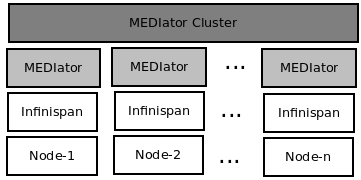
\includegraphics[width=0.6\textwidth]{deployment.png}
 }
\end{center}
 \caption{Deployment}
 \label{fig:deployment}
\end{figure}

The data replication and synchronization tool consists of 3 APIs, to be able to connect to specific data source, to integrate multiple data sources and meta data into the system, and to create replica sets for the data sources. While $PubConsAPI$ provides and manages a replica set for a specific data source, $Integrator$ integrates multiple data sources and provides a meta map and maps for each of the data sources to access the relevant information for each of the entry. Hence, while $PubConsAPI$ deals with the replica sets, $Integrator$ deals with meta data of multiple data sources. $InterfaceAPI$ is often provided by the data sources, as a mean to query and retrieve the data from the remote data sources.


The data replication and synchronization tool lets the users to create, update, retrieve, and delete replica sets, and share the replica sets with others. Replica sets are stored and processed in the Infinispan maps, where integrating with the data sources is done by the $InterfaceAPI$ interface. $Integrator$ interface provides a coarse granular integration with the data sources, letting the users to store meta data from multiple heterogeneous sources in a coarse grain access. 

Methods for RESTful invocations are designed for each of the interfaces defining the APIs. Methods that are defined in the interfaces should be implemented by the classes that implement these interfaces. Table~\ref{table:interfaces} depicts the methods defined for each of the interfaces

\begin{table}[!ht]
\centering
\caption{Methods defined for the Interfaces}
\label{table:interfaces}
\begin{tabular}{|c||c| |c|}

\toprule
\textbf{Data Source Management} & \multicolumn{2}{c}{\textbf{ReplicaSet Management}} \\
\midrule

\textbf{$InterfaceAPI$} & \textbf{$PubConsAPI$}&\textbf{$Integrator$} \\
\hline
retrieve & createReplicaSet&updateExistenceInDataSource \\
  & duplicateReplicaSet&doesExistInDataSource\\
  & getRawData&getRawData\\
 & getReplicaSet&getMetaData \\
 & putReplicaSet&putMetaData \\
 & updateReplicaSet&updateMetaData \\
 & deleteReplicaSet&deleteMetaData \\
\bottomrule
\end{tabular}
\end{table}

While the interfaces of $PubConsAPI$ and $Integrator$ look similar with some common methods, they differ on what they manage. 

\subsection{Generic Design}
Classes extending PubConsAPI design and implement the logic of replica sets management, where integration with the data sources is done by two interfaces - Interface API and Integrator. Interface API provides data retrieval from the data source, where Integrator integrates multiple data sources into the system and store the meta data of the data sources into Infinispan.

A generic design was created as an example implementing the Interface API and PubConsAPI.

Two distributed cache instances exist in InfDataAccessIntegration.
\begin{lstlisting}  
    protected static Cache userReplicasMap;
    protected static Cache replicaSetsMap;
\end{lstlisting}  
userReplicasMap is a mapping of userId \ding{213} Array of replicaSetIDs. UserID could be the logged in user name. (for now, testing with random strings).
replicaSetsMap is a mapping of replicaSetID \ding{213} replicaSet.

Though this could be replaced with a single cache instance with the mapping of userID \ding{213} replicaSets, having two cache instances will be more efficient during searches, duplicates, and push changes. Hence, two cache instances design was chosen.

$InfDataAccessIntegration$ implements the PubConsAPI for publisher/consumer, where $InterfaceManager$ implements the $InterfaceAPI$ for the interface between the data source and the data replication and synchronization tool. Invoker classes extending the abstract class InterfaceManager, implement the respective data source integration to invoke these methods. The execution flow is depicted by Figure~\ref{fig:execution}.

\paragraph*{multi-tenancy}
The Replication Tool is multi-tenanted, and it is aware of the multiple tenants or users using the system. Each user co-exist in the replication tool at the same time, without the knowledge of existence of the other users, sharing the same cache space. 

\paragraph*{DataProSpecs - PubConsAPI}
The methods of $DataProSpecs$ can be invoked by knowing the respective replicaSetID of the replica set and the user ID of the user who owns the replica set. User ID is a random string that is input by the user. Probably this can be some `secret' or pass from the user. userIDs serve as the keys of the userReplicasMap. Apart from that, there is no data structure to hold the list of users.

$createReplicaSet()$ requires the userID along with the elements to be stored in the replica set. It returns the $replicaSetID$, which is further used to uniquely identify the replica set. $getReplicaSet()$ requires only the relevant $replicaSetID$ to return the respective replica set. Similarly, $updateReplicaSet()$ requires $replicaSetID$ as well as the elements to be stored in the $replicaSet$, replacing the previous elements. $deleteReplicaSet()$ requires both the $userID$ and $replicaSetID$. Similarly, $duplicateReplicaSet()$ requires both $replicaSetID$ and the userID of the user to whom the replicaSet is shared to. Creating, deleting, and duplicating a replication set requires modification to the user replicas map, which holds the list of the replica sets for the particular user. Hence the necessity to input the userID. ReplicaSetID is a large negative number (UUID) randomly generated. It can be safely assumed to be harder to guess. Hence, this model is assumed to provide adequate security for this prototype.

\subsection{Integration with Multiple Data Sources}
Clinical data is deployed in multiple data sources such as TCIA, CA Microscope, and Amazon S3. Figure~\ref{fig:dsdeployment} depicts the deployment of the system with multiple data sources. A set of clinical data was uploaded to S3, where the meta data mapping of patientID \ding{213} fileName was available as a CSV file. Similarly CSV file depicting clinical information is available, as multiple properties against the UUID, such as patient ID. These files are parsed and stored into meta data maps in Infinispan. The CSV files containing meta data or $resource ID \ding{213} fileName$ mapping are stored locally in the file system or in a remote repository.
\begin{figure}[!htbp]
\begin{center}
 \resizebox{\columnwidth}{!}{
  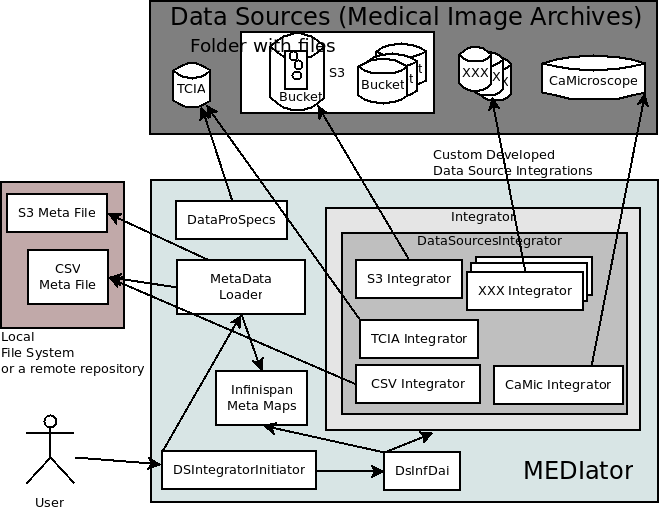
\includegraphics[width=\textwidth]{dsdeployment.png}
 }
\end{center}
 \caption{Deployment Diagram of the System and the Data Sources}
 \label{fig:dsdeployment}
\end{figure}

Each data source is connected to the replication tool by implementing a class that extends Integrator interface. DatasourcesIntegrator is an abstract class implementing the common features of the currently implemented 4 data sources - CSV, CA Microscope, S3, and TCIA. CsvIntegrator, CaMicIntegrator, S3Integrator, and TciaIntegrator respectively implement the integrators for each of these data sources. $MetaDataLoader$ loads the CSV files and stores them into Infinispan maps, against the ID, such as the patient ID. TciaIntegrator invokes TciaInvoker to retrieve the images and meta data from TCIA.

$DSInfDai$ a class extending $InfDataAccessIntegration$ holds the instances of map to store all the meta data. $DSIntegratorInitiator$ invokes the instances of $DSInfDai$, $MetaDataLoader$ and the other respective classes to start parsing the meta data, and store the instances into the respective maps. Figure~\ref{fig:dsclass} represents the class diagram of data source integrators, along with the 3 interfaces of the replication tool.

\begin{figure}[!htbp]
\begin{center}
 \resizebox{\columnwidth}{!}{
  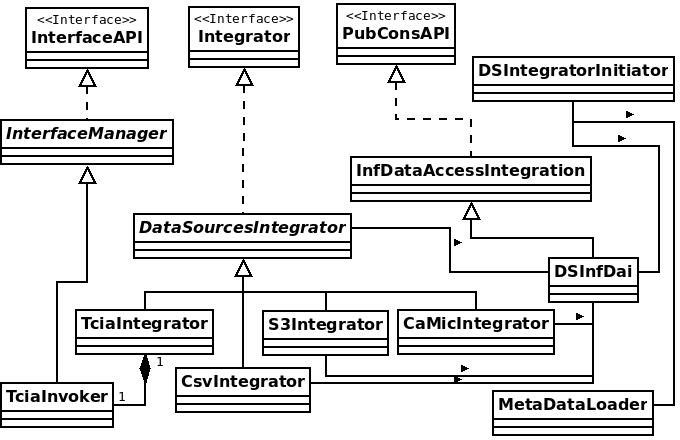
\includegraphics[width=\textwidth]{dsclass.png}
 }
\end{center}
 \caption{Class Diagram of data sources integrators along with the higher level API}
 \label{fig:dsclass}
\end{figure}

\begin{lstlisting}  
    protected static Cache<String, Boolean[]> metaMap; /*csv, ca, tcia, s3*/
    protected static Cache<String, String[]> csvMetaMap;
    protected static Cache<String, String> s3MetaMap;
    protected static Cache<String, String> caMetaMap;
\end{lstlisting} 
The $metaMap$ stores a binary array against each of the key (such as, patientID) to point the existence of meta data in the data sources defined, in this case, CSV, CA Microscope, TCIA, and S3. $s3MetaMap$ provides the file name for the respective ID, which can be used to find the location of the file as it follows the pattern of of $S3\_BASE\_URL + folderName + ``/'' + fileName$. Similarly, $caMetaMap$ stores the URL that the respective object is stored. $csvMetaMap$ contains the meta data loaded from the CSV files against the respective ID.

Methods for updating, creating, and deleting meta data from these maps are available where creating or deleting meta data will update the availability to true/false for the respective index in the $metaMap$. $XXX\_META\_POSITION$ defines the position in the metaMap, where XXX stands for CSV, CA, TCIA, and S3. Updating the existence will flop the respective boolean value in the respective entry. The $metaMap$ ensures easy indexing, and helps to search which of the data sources contain the respective information for any given key, such as a given patient ID.


\subsection{Software Architecture}
Figure~\ref{fig:arch} depicts the architecture of the data replication and synchronization tool, showing its components and dependencies.
\begin{figure}[!htbp]
\begin{center}
 \resizebox{0.5\columnwidth}{!}{
  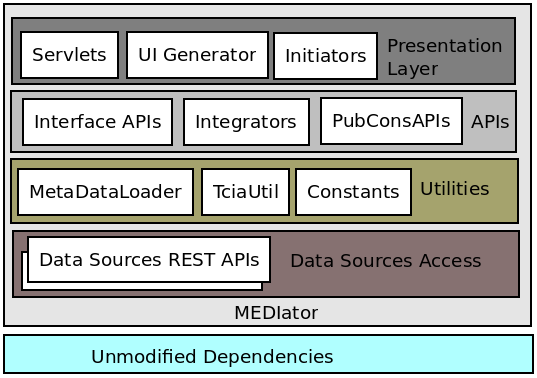
\includegraphics[width=0.5\textwidth]{arch.png}
 }
\end{center}
 \caption{Architecture}
 \label{fig:arch}
\end{figure}

Dependencies are used unmodified. Dependencies such as Apache HTTP Client and Mashape Unirest are configured and leveraged by the InteraceAPI, to query and retrieve the raw data from the data sources. Infinispan, as the core dependency, is configured and exploited as the shared storage and distributed execution medium. Presentation layer dependencies such aS Embedded Tomcat, Apache Velocity, and Log4j2 facilitate prototype application development with web pages, and configurable logging. Apache Maven is used as the project management dependency to build, deploy, and execute the project effectively.

Data sources access layer consists of means of accessing the data sources, such as querying and downloading the data stored in Amazon S3 or TCIA, via the REST API. Utilities such as MetaDataLoader and TciaUtil provide utility methods and functionalities for the tool throughout its execution.

InterfaceAPIs, Integrators, and PubConsAPIs are implemented at the top level, extending their respective base classes. The presentation layer consists of the Intiiators that function as the starting point of the prototype applications. Servlets and UI Generators generate the presentation layer of the tool.

\section{Implementation}
Different complex data sources require custom development extending the generic framework. As creating and customizing the replicaSet require a more specific data structure, further implementations are done, extending the core class hierarchy\footnote{The source code can be accessed from \url{https://bitbucket.org/BMI/datareplicationsystem}}. 

\subsection{Generic Implementation}
Base classes of the APIs were implemented to provide a generic synchronization tool, that stores the entire search queries of any data source as the replica set. When the user logs in, $logIn()$ checks whether the user has already stored replicaSets from the Infinispan distributed Cache. If so, execute them all again. This would be changed later as we do not have to execute all. Rather, we need to execute for the diffs. When the user performs new searches, for the images, series, collections, and the other meta data, the results will be returned to the user, and the user can chose ta subset of the returned results to create a replicaSet.
\begin{figure}[!htbp]
\begin{center}
 \resizebox{\columnwidth}{!}{
  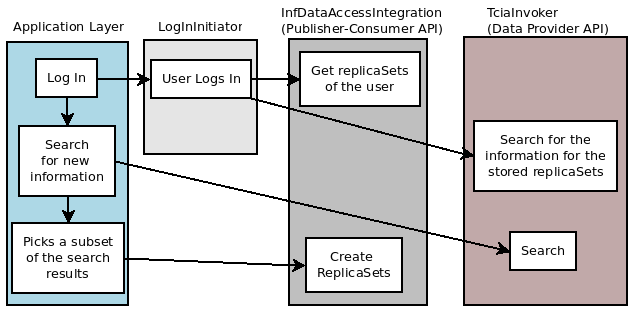
\includegraphics[width=\textwidth]{execFlow.png}
 }
\end{center}
 \caption{Execution Flow}
 \label{fig:execution}
\end{figure}
The replicaSet for the image will be as,
\begin{lstlisting}  
TCIAConstants.IMAGE_TAG + "getImage?SeriesInstanceUID=" + seriesInstanceUID
\end{lstlisting}  
For other information (meta data), such as collections and seies,
\begin{lstlisting}  
TCIAConstants.META_TAG + query;
\end{lstlisting}  

Here, query takes the below format. 
\begin{lstlisting}  
"getSeries?format=" + format +
                "&Collection=" + collection +
                "&PatientID=" + patientID +
                "&StudyInstanceUID=" + studyInstanceUID +
                "&Modality=" + modality;
\end{lstlisting}  
When a new instance starts now, and invokes the log in action for the same user, it will execute the queries for the stored replicaSets again, and reproduce the same results.

\subsection{TCIA Implementation}
An extension based on the base design was developed for TCIA, as shown by Figure~\ref{fig:class}, which provides a core class hierarchy of the system.
\begin{figure}[b]
\begin{center}
 \resizebox{0.8\columnwidth}{!}{
  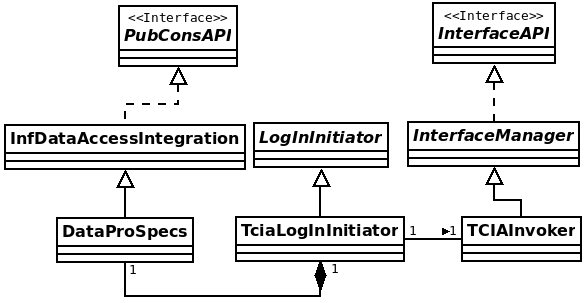
\includegraphics[width=0.8\textwidth]{classDiagram.png}
 }
\end{center}
 \caption{Core Class Hierarchy}
 \label{fig:class}
\end{figure}

\paragraph*{TciaInvoker - Interface API}
$TciaInvoker$ extends $InterfaceManager$ to implement the interfacing layer between the TCIA data source and the data replication and synchronization tool. Meta data such as collections, patients, studies, and series are retrieved at different levels, though the default download manager of TCIA downloads the data in series level, composed of the images of the series in a single zip archive. While having the default userReplicasMap to contain the IDs of the replica sets for each user, the replica set itself is stored in multiple maps instead of a single replicaSets map, to provide an efficient storage and access.

$DataProSpecs$ extends the $InfDataAccessIntegration$ class. 5 maps are created as below to represent the replica sets.
\begin{lstlisting}  
    protected static Cache<Long, Boolean[]> tciaMetaMap;
    protected static Cache<Long, String[]> collectionsMap;
    protected static Cache<Long, String[]> patientsMap;
    protected static Cache<Long, String[]> studiesMap;
    protected static Cache<Long, String[]> seriesMap;
\end{lstlisting} 

$tciaMetaMap$ contains a boolean array, which reflects which of the granularity of meta data is selected as a whole. For TCIA, if a few collections are selected, the first element of the array is set to true, and similarly, the other meta data are marked to true or false as shown by the below code segment.
\begin{lstlisting}  
        Boolean[] metaMap = new Boolean[4];
        metaMap[0] = collection != null;
        metaMap[1] = patientID != null;
        metaMap[2] = studyInstanceUID != null;
        metaMap[3] = seriesInstanceUID != null;

        putReplicaSet(replicaSetId, metaMap);
\end{lstlisting} 
The name of the collections, patientID, studyInstanceUID, and seriesInstanceUID are stored against the respective replicaSetID in collectionsMap, patientsMap, studiesMap, and seriesMap respectively. Hence changes are done at the respective maps. Duplicating the replicaSets duplicate the contents of the entire row to a new replicaSetID. Similarly, deleting a replicaSet deletes the respective information from all the maps.

TCIA public API provides methods to retrieve the images and meta data of different granularity. Figure~\ref{fig:methods} depicts the methods that retrieve image and metadata at different granularity from TCIA. These methods are invoked by the replication manager tool to retrieve the images. As shown by Figure~\ref{fig:methods} an initial search on TCIA may contain parameters such as modality, in addition to collection name, patient ID, study instance ID, and series instance UID. However, each of these search returns the output in a finer granularity, and when a sub set of this finer granularity is selected, each of the selected elements are always identified by their respective identifier. Hence, storing an array of patient ID would be sufficient to identify the selected sub set of the collection including the array of patients. Similary an array of study instance UID is sufficient to represent the selected sub set of any patient, and an array of series instance UID is sufficient to represent the selected sub set of any study, as it will contain an array of series.

\begin{figure}[!h]
\begin{center}
 \resizebox{\columnwidth}{!}{
  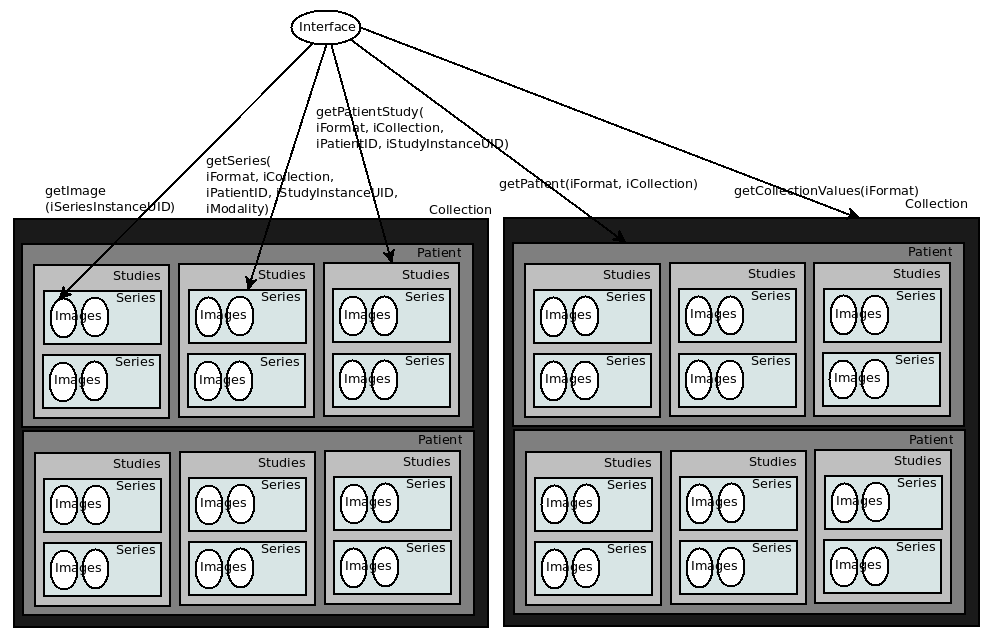
\includegraphics[width=\textwidth]{methods.png}
 }
\end{center}
 \caption{Retrieving images and meta data}
 \label{fig:methods}
\end{figure}



\section{Evaluation}
A prototype web application was built with the data replication and synchronization tool and TCIA REST API. Apache Velocity was used to generate the web pages for the replication tool. Apache Tomcat (Embedded) was integrated into the program such that it will get the user inputs from the HTML pages and present the output in pages formatted by Apache Velocity Templates. Respective servlets were created inside the servlets package to receive the inputs from HTML pages to the backend Java code.

$DataRetriever$ class is invoked to retrieve the meta data from TCIA and to create and retrieve replica sets. $UIGenerator$ class invokes the Apache Velocity templates to create the web pages, presenting the data to the users. $DataRetriever$ has instances of $TciaInvoker$ and $TciaLogInInitiator$ to invoke the TCIA queries and replication tool create and retrieve replicaSets mechanisms. $TciaLogInInitiator$ has instances of $TciaInvoker$ and $DataProSpecs$, to invoke the public APIs provided by these classes for the data provider specification and publisher/consumer APIs. Figure~\ref{fig:classUX} depicts the class hierarchy involved in the user interface.
\begin{figure}[!htbp]
\begin{center}
 \resizebox{0.55\columnwidth}{!}{
  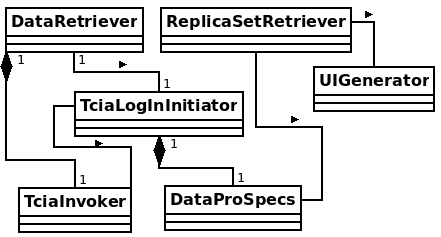
\includegraphics[width=0.55\textwidth]{classUX.png}
 }
\end{center}
 \caption{Class Hierarchy of the User Interface}
 \label{fig:classUX}
\end{figure}

\section{Conclusion}
\balance
Storing a selected sub set of data items that matches a specific criteria as a replica set is an optimal way to bookmark large data sources. Users should be able to create and update their replica sets, and share it with others using a unique identifier. While different data sources have different interfaces, a generic data replication and synchronization tool will be convenient, such that sharing of replica sets across heterogeneous data sources will be possible. This project researched the possibilities of such a replication and data synchronization tool, exploiting the in-memory data grid projects, and implements a data synchronization and replication tool with Infinispan while consuming data sources such as TCIA via their public APIs.

\section{Future Work}
\paragraph*{Get the Raw Images}
$getRawData(String key)$ method should be implemented in the classes implementing the $PubConsAPI$ and $Integrator$ interfaces to be able to download the raw data from the data sources such as TCIA, CA Microscope, or S3, for the given replica set, potentially using Java web start.

\paragraph*{Tracking the downloaded items}
Consumers download the data by searching the image repository using the browser. The information that the consumer is interested in, gets updated whenever the data producers update or add patient information. The current download tool lacks the ability to track the relevant updates to the consumer. A data replication and synchronization tool will assist automated downloads to the consumers. Users can create replica sets as a sub set of their search queries, and share their replica sets with other users, and update their replica sets periodically. Replica sets can be used as a way of tracking and sharing information.

Currently, when a user initates download of a replica set, finishes the download, and later restart the download, the download mechanism still would download the whole replica set again, as there is no track of what has already been downloaded. A sample timeline of the events is given below.\\
 $t_{0}$: \textit{User A} Creates Replica Set $R_{1}$ with a query.\\
 $t_{1}$: \textit{User A} accesses and downloads the contents of the replica set $R_{1}$ and finds the contents to be ${A,B,C}$.\\
 $t_{2}$: The contents matching the replica set $R_{1}$ query modified to be ${A,B,D}$ by an outside event such as more images added and existing images removed.\\
 $t_{3}$: \textit{User A} downloads the contents of $R_{1}$ again.

This should be designed such that the already accessed images would not be downloaded while the newly available or not previously accessed segments of the replica set will be downloaded. For example, in the above scenario, currently at $t_{3}$, all A, B, and D will be downloaded, where an implementation should allow only the new or modified contents to be downloaded.

\paragraph*{Security}
The data replication and synchronization can be further secured with user authentication. SAML tokens can be created for user names and passwords with the membership information. The SAML tokens can be validated later. A create and validate API with user stores such as LDAP or OpenID should be designed and implemented, extending and leveraging the replication tool.

\subsection{Developer Guide}
This section describes how the future work could be done.

Replica sets management is handled by both $Integrator$ and $PubConsAPI$ interfaces. If multiple data sources should be managed consecutively, having maps pointing to meta data from heterogenous sources, $Integrator$ interface should be implemented in a class with the respective distributed maps to hold the meta data. If a single data source is involved with a fine grain control over a data source, $PubConsAPI$ should be implemented. Functionality such as security with SAML token should be implemented as an Integrator, as this involves SSO for multiple data sources.

Similarly, involving a time stamp for the class extending $PubConsAPI$, downloaded items can be tracked, and the diffs can be produced for the user download.

$InterfaceAPI$ integrates the tool with the data source, such that the relevant data can be queried, searched, manipulated, and downloaded. Hence, respective classes should implement this interface for each of the data source. The TCIA integration by the $tcia\_rest\_api$ package stands as a decent sample on implementing this interface.

%\begin{thebibliography}{1}
%\end{thebibliography}

\end{document}


